%\renewcommand{\cftfigpresnum}{Lampiran }
%\renewcommand{\thetable}{\arabic{chapter}.\arabic{table}}   
 \chapter{Lampiran}
 %\section{•}
  %\setcounter{table}{A}
 	\counterwithin{figure}{chapter}  
   \begin{figure}[H]
   \centering
  	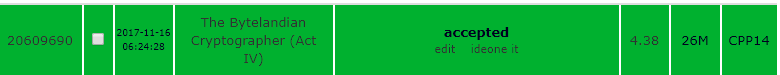
\includegraphics[scale=0.53]{images/lampiran/best.png}
  	\caption{Hasil Uji Coba pada Situs Penilaian SPOJ}
  	\label{fig:best_submission}
  	\end{figure}
	
	 \begin{figure}[H]
  \centering
  	 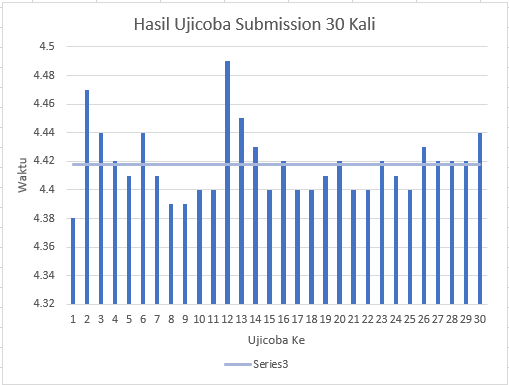
\includegraphics[scale=0.7]{images/lampiran/uji31.png}
  	\caption{Grafik Hasil Uji Coba pada Situs SPOJ Sebanyak 30 Kali}
  	\label{fig:chart}
  \end{figure}  	
  	
  	\begin{figure}[H]
  	\centering
  	 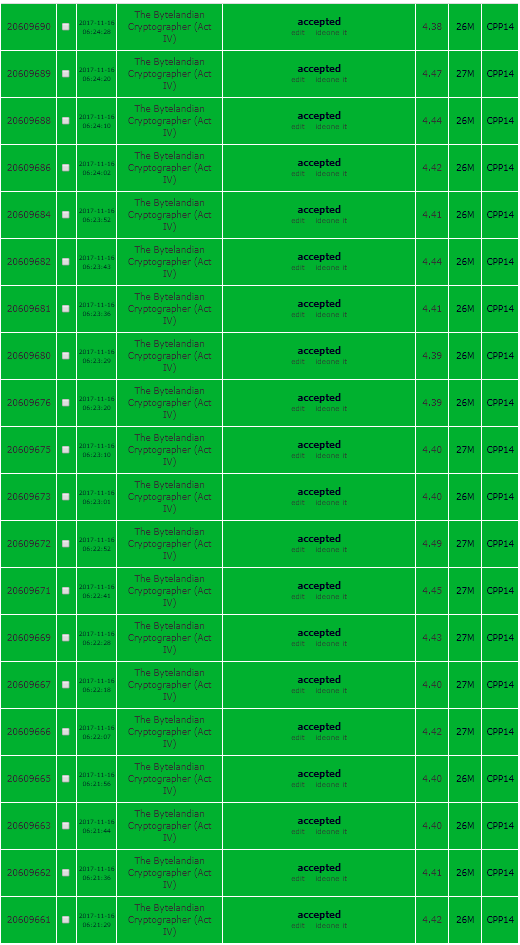
\includegraphics[scale=0.63]{images/lampiran/uji1.png}
  	\caption{Hasil Pengujian Sebanyak 30 Kali pada Situs Penilaian Daring SPOJ (1)}
  	\label{fig:submission1}
  \end{figure}
  
  \begin{figure}[H]
  \centering
  	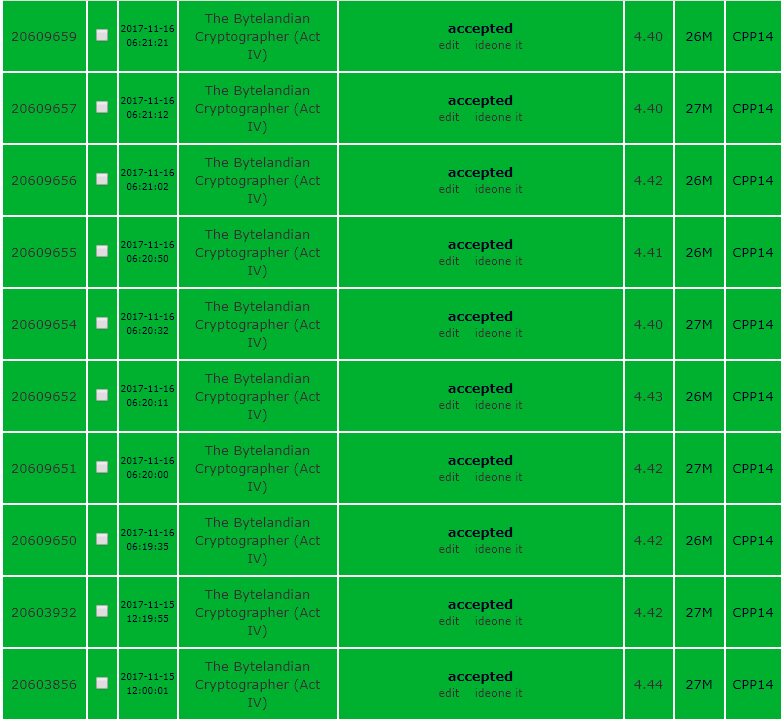
\includegraphics[scale=0.5]{images/lampiran/uji3.png}
  	\caption{Hasil Pengujian Sebanyak 30 Kali pada Situs Penilaian Daring SPOJ (2)}
  	\label{fig:submission2}
  \end{figure}
  
  \begin{figure}[H]
  \centering
  	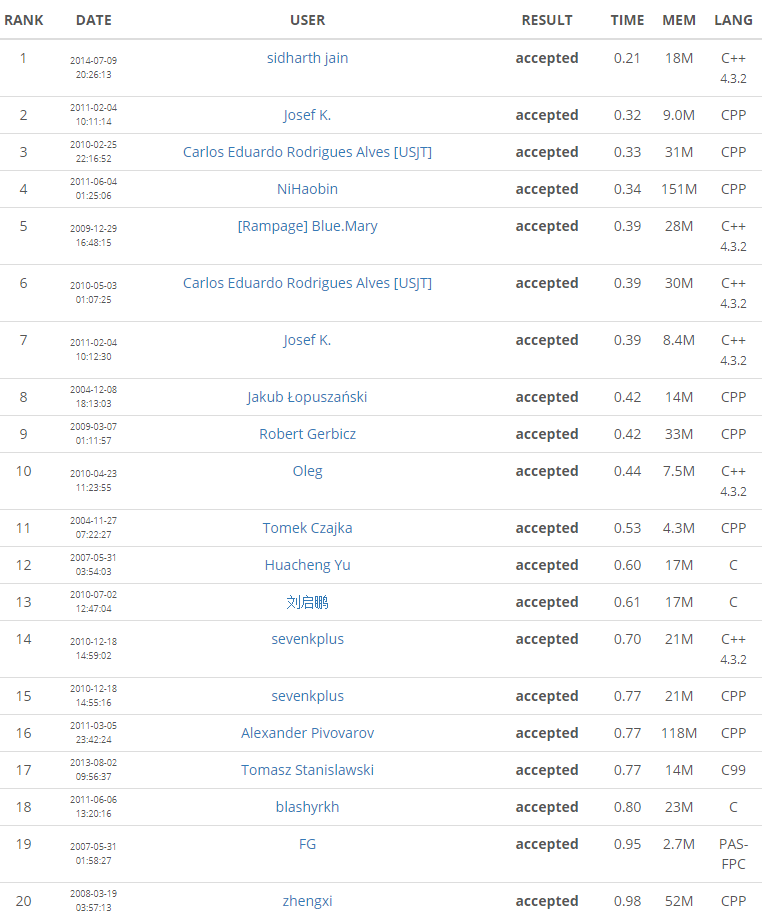
\includegraphics[scale=0.55]{images/lampiran/rankdiatas1.png}
  	\caption{Daftar Peringkat Berdasarkan Kecepatan yang Diperoleh dari Dari SPOJ(1)}
  	\label{fig:per1}
  \end{figure}
  
  \begin{figure}[H]
  \centering
  	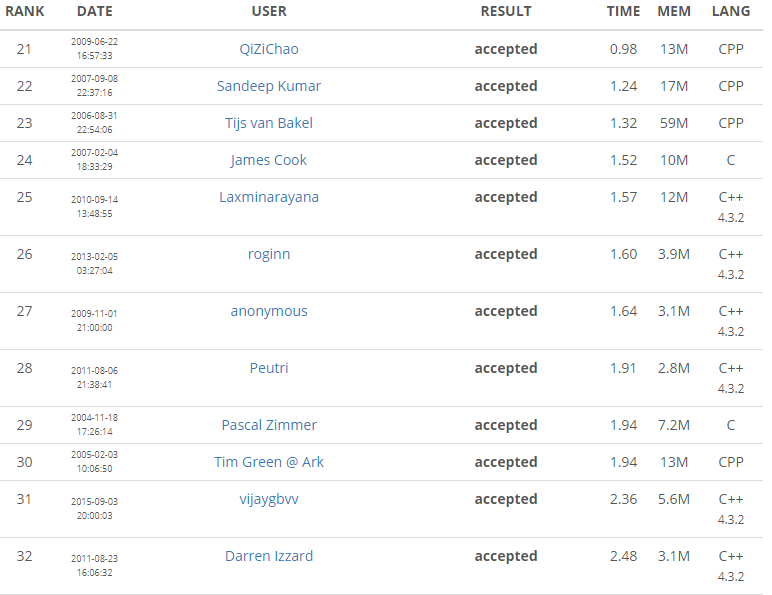
\includegraphics[scale=0.55]{images/lampiran/rankdiatas2.png}
  	\caption{Daftar Hasil Peringkat Berdasarkan Kecepatan yang Diperoleh dari Dari SPOJ(2)}
  	\label{fig:per2}
  \end{figure}
  
